\documentclass[14pt,a4paper]{extarticle}
\renewcommand{\abstractname}{Аннотация}
\usepackage[margin=1in]{geometry}

\usepackage[russian]{babel}
\usepackage{fontspec}

\usepackage{amsmath}
\usepackage{graphicx}
\usepackage{xcolor}
\usepackage{unicode-math}

% Настройка блоков
\usepackage[most]{tcolorbox}
\newtcolorbox{solutionbox}[1]{
	enhanced,
	colback=blue!5!white,      % Цвет фона
	colframe=blue!75!black,    % Цвет рамки
	fonttitle=\bfseries,
	title={#1},                % Заголовок блока
	attach boxed title to top left={xshift=5mm, yshift=-3mm},
	boxed title style={colback=blue!75!black},
	sharp corners,             % Острые углы (можно убрать для скругления)
	drop shadow,               % Тень
	breakable                  % Чтобы блок переносился на другие страницы
}

% Настройка библиографии
\usepackage{csquotes}
\usepackage[
backend=biber,
style=gost-numeric,
sorting=none
]{biblatex}
\addbibresource{refs.bib}

\usepackage{microtype}

\usepackage[outputdir=build]{minted}
\usemintedstyle{colorful}
\setminted{
    fontsize=\small,
    breaklines,
    frame=lines,
    tabsize=4
}

\setmainfont{STIX Two Text}
\setmathfont{STIX Two Math}
\setmonofont{JetBrains Mono}[Scale=MatchLowercase]

\usepackage[unicode,colorlinks=true,linkcolor=black!65!blue,citecolor=black!65!blue,urlcolor=black!65!blue]{hyperref}

\setlength{\parindent}{1.25cm}
\setlength{\parskip}{0.5\baselineskip}

\newcommand{\refneed}{{\color{red} ТРЕБУЕТСЯ ССЫЛКА}}

\begin{document}
\hypersetup{pageanchor=false}
\begin{titlepage}
\thispagestyle{empty}

\begin{center}
\vspace*{0.8cm}

\includegraphics[width=0.6\textwidth]{assets/logo.png}
\end{center}

\vspace{1.4cm}

\noindent
{\large \textbf{Выпускная квалификационная работа}}\par

\vspace{1.1cm}

\noindent
{\large \textbf{Тема работы}}\par
\vspace{0.35cm}
{\noindent \LARGE \bfseries Создание цифровых двойников\par}
{\noindent \LARGE \bfseries с использованием технологии\par}
{\noindent \LARGE \bfseries Gaussian Splatting\par}

\vfill

\begin{flushright}
\begin{minipage}{0.3\textwidth}
{\large \textbf{Автор}}\par
Володченков\par
Никита Дмитриевич\par
\vspace{0.8cm}

{\large \textbf{Группа}}\par
А-05-22\par
\vspace{0.8cm}

{\large \textbf{Руководитель}}\par
Кожевников\par
Антон Вадимович\par
\vspace{0.8cm}

{\large \textbf{Дата}}\par
\today
\end{minipage}
\end{flushright}

\vfill

\end{titlepage}
\clearpage

\begin{abstract}
	Данная выпускная квалификационная работа посвящена разработке пайплайна для создания интерактивных цифровых двойников на основе воксельных медицинских данных. Традиционные методы визуализации КТ и МРТ, такие как прямой объемный рендеринг, требуют значительных вычислительных ресурсов для работы в реальном времени. В качестве альтернативы в работе исследуется применимость современной технологии 3D Gaussian Splatting (3DGS), которая позволяет совместить высокую скорость отрисовки с фотореалистичным качеством, что делает ее перспективным решением для прикладных медицинских и образовательных задач.
	
	\textbf{В целях исследования} был спроектирован процесс обработки данных на примере костной системы человека из анатомического набора данных Visible Human Project (сегментированного и очищенного другими исследователями). Разработанные скрипты преобразуют исходную сетку вокселей в формат OpenVDB для последующей генерации выборки ракурсов в графическом редакторе Blender. Интеграция процесса обучения с библиотекой gsplat обеспечивается за счет автоматического формирования конфигурационных файлов виртуальных камер в формате COLMAP, затем обученные трехмерные гауссианы сегментируются по принципу ближайшего соседа на основе исходной размеченной воксельной сетки.
	
	\textbf{Практическим результатом работы} стала фотореалистичная модель скелета человека и адаптированный под нее интерактивный браузерный просмотрщик на базе WebGL, где реализована функция динамического выделения цветом выбранного класса.
\end{abstract}
\clearpage

\hypersetup{pageanchor=true}
\setcounter{page}{2}
\tableofcontents
\clearpage

\section{Прямой объемный рендеринг}
\subsection{Уравнение переноса излучения}

Объемный рендеринг строится на дифференциальном уравнении, описывающем поведения света в среде и называемым Уравнением переноса излучения. В наиболее общем виде оно формулируется следующим образом:
%
\begin{equation}
	\label{eq:phys_rte}
	\frac{\mathrm dI_\nu}{\mathrm ds} = - \alpha_\nu I_\nu + \varepsilon_\nu,
\end{equation}
%
где $I_\nu$ - текущая интенсивность излучения на частоте $\nu$, $\alpha_\nu$ - коэффициент поглощения, $\varepsilon_\nu$ - коэффициент излучения.

Численным решением уравнения занимаются различные движки рендеринга, например работа \cite{pbrt}, которая использовалась для написания теории настоящего раздела.

В компьютерной графике принято интенсивность излучения обозначать за $L$, а преодоленное расстояние за $t$. Не ограничивая общности, далее рассматривается конкретная частота $\nu$, которая в формулах будет опускаться.

Частица света, попадая в объем, может встретить частицу среды и:
%
\begin{enumerate}
	\item быть поглощенной ею (absorption);
	\item перенаправленной в другую или с некоторой вероятностью в ту же сторону (scattering);
	\item частица света вообще может не встретиться с объемом и пролететь дальше без изменений.
\end{enumerate}
%
В точке $\mathrm p$ свет, приходящий из направления $-\omega$ и равный $L_i(p, -\omega)$, в силу поглощения выйдет с интенсивностью $L_o(p, \omega)$ не весь. Описать изменение интенсивности света в силу поглощения можно с помощью величины коэффициента поглощения: $\sigma_a$:
%
\begin{equation}
	\label{eq:dl_absorption}
	\mathrm dL(\mathrm p, \omega) = L_o(\mathrm p, \omega) - L_i(\mathrm p, -\omega) = -\sigma_a(\mathrm p, \omega) L_i(\mathrm p, -\omega) \mathrm dt.
\end{equation}
%
Каждая поглощенная частица отдает объему какую-то энергию, и для сохранения равновесия объем может сам начать излучать свет. Таким образом, влияние собственного излучения объема на итоговый свет может быть выражено как:
%
\begin{equation}
	\label{eq:dl_emission}
	\mathrm dL(p, \omega) = \sigma_a(\mathrm p, \omega) L_e(\mathrm p, \omega) \mathrm dt,
\end{equation}
%
где $L_e$ это также собственное свойство объёма, задаваемое зараннее, либо в художественных целях можно задать, что $\mathrm dL(p, \omega) = \mathrm{const}$ (здесь подразумевается вклад только собственного излучения).

Упомянутое равнее рассеяние несет вклад в итоговый свет с двух противоположных сторон. Если поступающее излучение $L_i$ подвергается рассеянию, оно перенаправляется объемом по некоторому распределению $p(\omega, \omega')$. $p$ называется фазовой функцией и задает для каждого входящего света с направления $\omega$ плотность распределения на сфере $S^2$ для выходящих направлений $\omega'$, то есть:
\[
	\int_{S^2} p(\omega, \omega') \mathrm d\omega' = 1.
\]
С одной стороны, если бы объема не было, любой приходящий свет $L_i(\mathrm p, -\omega)$ мог быть нетронутым, но в силу рассеяния, может изменить свое направление, отрицательно повлияв на выходящий свет $L_o(\mathrm p, \omega)$. Это можно описать с помощью коэффициента рассеяния $\sigma_s$:
%
\begin{equation}
	\label{eq:dl_outscattering}
	\mathrm dL(\mathrm p, \omega) = -\sigma_s(\mathrm p, \omega) L_i(\mathrm p, \omega) \mathrm dt
\end{equation}
%
Это же явление может перенаправить весь входящий с других направлений $\omega_i$ свет в рассматриваемую сторону, положительно повлияв на выходящий свет $L_o(\mathrm p, \omega)$:
%
\begin{equation}
	\label{eq:dl_inscattering}
	\mathrm dL(\mathrm p, \omega) = \sigma_s(\mathrm p, \omega) \left( \int_{S^2} p(\mathrm p, \omega_i, \omega) L_i(\mathrm p, \omega_i) \mathrm d\omega_i \right) \mathrm dt
\end{equation}
%
С наблюдениями \ref{eq:dl_absorption}, \ref{eq:dl_emission}, \ref{eq:dl_inscattering}, \ref{eq:dl_outscattering}, уравнение \ref{eq:phys_rte} может быть переписано в следующей форме:
%
\begin{equation}
	\label{eq:graphics_rte}
	\frac{\mathrm dL}{\mathrm dt} = -\sigma_t L + \sigma_s L_s + L_e,
\end{equation}
%
где $\sigma_t = \sigma_a + \sigma_s$ (коэффициент экстинкции, описывающий вероятность встретить частицей света частицу среды, или ещё это означает, что в среднем частице понадобится пролететь расстояние $\sigma_t^{-1}$ чтобы встретить частицу среды), $L_s$ соответствует интегралу из уравнении \ref{eq:dl_inscattering}, а $L_e$ уже содержит в себе $\sigma_a$ из уравнения \ref{eq:dl_emission}.

Подходы к решению уравнения, от быстрых, но неточных решений, до медленных, но сильно приближенных к точному решению, будут описаны в оставшихся разделах про прямой рендеринг.
\subsection{Решения для рендеринга в реальном времени}
\label{sec:raycasting_splatting}

Как было выяснено в предыдущем разделе, для осуществления рендеринга требуются знания о свойствах среды во всех её точках. Эти данные задаются на обыкновенной воксельной сетке.

Для быстрой визуализации объемных данных удобно считать, что рассеивание отсутствует, так как из-за него возникают трудно отслеживаемый in-scattering. Если принять $\sigma_a=\sigma$, $\sigma_s=0$, уравнение \ref{eq:graphics_rte} упрощается до
%
\[
	\frac{\mathrm dL}{\mathrm dt} = -\sigma L + L_e.
\]
%
Решение уравнения приводится в работе \cite{max1995optical}, из которой
%
\begin{equation}
	\label{eq:int_rte_emm_abs}
	L(t) = L(0)e^{-\tau(t)} + \int_0^t L_e(s) e^{-\tau(s)} ds,
\end{equation}
%
\[
	\tau(t) = \int_0^t \sigma(s) ds.
\]

\begin{figure}[ht]
	\centering
	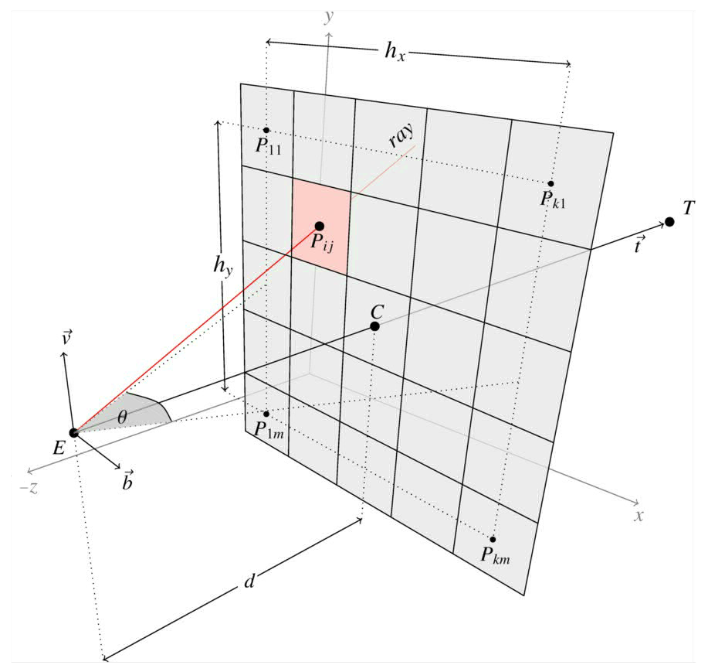
\includegraphics[width=0.5\textwidth]{assets/ray-casting.png}
	\caption{Пример испускания лучей через центры всех пикселей изображения (метод Ray Casting).}
	\label{fig:ray_casting}
\end{figure}

\textbf{Ray casting}. (рисунок \ref{fig:ray_casting}) Луч можно представить как
%
\[
	\mathrm r(t) = \mathrm o + t\mathrm d,
\]
%
где $\mathrm o$ - центр камеры, $\mathrm d$ - единичный вектор, соединяющий центр камеры и центр соответствующего пикселя. Первый метод численного решения уравнения \ref{eq:int_rte_emm_abs} заключатся в испускании лучей из камеры (наблюдателя) через каждый пиксель проективной плоскости. C использованием метода конечных разностей вдоль луча $r$ с шагом $\Delta t$ вычисляется приблизительный ответ. Оказывается удобным ввести непрозрачность
%
\begin{equation}
	\label{eq:rc_transparency}
	1 - \alpha_i = e^{-\sigma(i\Delta t)\Delta t},
\end{equation}
%
которую удобней просчитать заранее\footnote{Стоит держать в голове, что непрозрачность зависит от величины шага и при его изменении потребует пересчета.}, как это уже было сделано с помощью функции переноса. Формула аккумулирования цвета (её также называют альфа-блендингом) имеет вид:
%
\begin{align}
	\label{eq:alpha_blending1}
	C^i_\text{acc} &=
		C^{i-1}_\text{acc} +
		(1 - \alpha^{i-1}_\text{acc}) (\alpha_i c_i); \\
	\label{eq:alpha_blending2}
	\alpha^i_\text{acc} &=
		a^{i-1}_\text{acc} +
		(1-\alpha^{i-1}_\text{acc}) \alpha_i,
\end{align}
%
где $c_i, \alpha_i$ вычисляются в точке $\mathrm o + i\Delta t \mathrm d$.

\begin{figure}[ht]
	\centering
	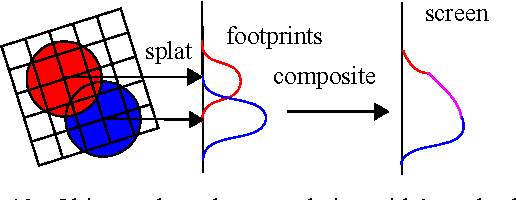
\includegraphics[width=0.5\textwidth]{assets/splatting.png}
	\caption{Ортографическая проекция гауссиан на экран (метод Splatting). Красним и синим здесь обозначены ядра, которыми заменены каждые воксели.}
	\label{fig:splatting}
\end{figure}

\textbf{Splatting}. (рисунок \ref{fig:splatting}) Вместо того, чтобы испускать лучи из камеры предлагается другой подход: проецировать воксели на камеру. В оригинальной статье, предложившей его \cite{westover1990footprint}, каждый воксель заменяется на функцию $h$ (ядро), что позволяет считать цвет и прозрачность каждой точки объема $(x, y, z)$ как
%
\[
	C(x, y, z) = \sum_i h(x-x_i, y-y_i, z-z_i) c_i,
\]
\[
	\alpha(x, y, z) = \sum_i h(x-x_i, y-y_i, z-z_i) \alpha_i.
\]
%
Суммирование ведется по всем вокселям, $(x_i, y_i, z_i), \alpha_i, c_i$ - координата центра, непрозрачность и цвет вокселя $i$ соответственно.

Конечно, у такого объема можно как и раньше вычислить изображение на экране методом ray casting, однако предлагается проецировать ядра на экран. В оригинальной статье модель проецирования --- ортографическая\footnote{Ортографическая проекция предполагает испускать лучи из центров каждого пикселя перпендикулярно плоскости изображения, в отличие от перспективной, где лучи испускаются из оптического центра камеры и проходят через центры пикселей.}, при этом не ограничивая общности лучи можно считать параллельнными $(0, 0, 1)$. Для ядра можно просчитать его влияние на луч, исходящий из $(x,y)$. Если просчитать все возможные лучи из плоскости $Oxy$, то получится двумерный отпечаток ядра
%
\begin{equation}
	h^i_\text{footprint} (x, y) = \int_{-\infty}^{+\infty} h(x-x_i, y-y_i, z-z_i) \mathrm dz.
	\label{eq:footprint}
\end{equation}
%
Непрозрачность и цвет каждого вокселя для текущего отрисовываемого пикселя пропорционально отпечатку. Учитывая удаленность центров ядер от плоскости, итоговое изображение можно получить по ранее выведенным формулам альфа-блендинга \ref{eq:alpha_blending1} и \ref{eq:alpha_blending2}.

Splatting с ядром Гаусса являются основоположниками 3D Gaussian Splatting, который подробно рассматривается в разделе \ref{sec:3dgs}.
\subsection{Трассировка лучей методом Монте-Карло}

Если учитывать рассеивание среды, то явно получить решение не представляется возможным. Поэтому метод Монте-Карло честно просчитывает поведение луча.

Простейшая идея заключается в том, чтобы испускать из всех источников света лучи, смотреть как они будут себя вести, и если они попадают на сенсор наблюдения, накапливать их, и таким образом получить изображение. Однако, вероятность случайно наблюдаемого луча попасть на сенсор крайне мала. Поэтому куда практичней идти от конца луча к его началу, в этом и заключается метод Монте-Карло.

В уравнении \ref{eq:graphics_rte} удобней выделить потери и прирост света:
%
\[
	\frac{\mathrm dL(\mathrm p, \omega)}{\mathrm dt} = 
	-\sigma_t(\mathrm p, \omega) L(\mathrm p, \omega) +
	S(\mathrm p, \omega),
\]
%
где
%
\[
	S(\mathrm p, \omega) =
	\sigma_a(\mathrm p, \omega) L_e(\mathrm p, \omega) + 
	\sigma_s(\mathrm p, \omega) \int_{S^2} p(\mathrm p, \omega', \omega) L(\mathrm p, \omega') \mathrm d\omega'.
\]
%
По аналогии с непрозрачностью, введенной для получения уравнения \ref{eq:int_rte_emm_abs}, вводится коэффициент пропускания
%
\[
	T(\mathrm p_1, \mathrm p_2) =
	e^{-\int_{\mathrm p_1}^{\mathrm p_2} \sigma_t(s) \mathrm ds}.
\]

Рассматривается конкретный луч $\mathrm r(t) = \mathrm o + t\omega$). Для того, чтобы не нагромождать формулы, далее $L(t, \omega)=L(r(t), \omega)$. Итоговое интегральное решение (доказательство приводится в \cite{max1995optical}) имеет вид:
%
\begin{align*}
	L(0, \omega) = T(0, d) L(d, \omega) + \int_0^d T(0, t) S(t, \omega) \mathrm dt, \\
	S(t, \omega) =
	\sigma_a(t, \omega) L_e(t, \omega) +
	\sigma_s(t, \omega) \int_{S^2} \mathrm p(t, \omega', \omega) L(t, \omega') \mathrm d\omega'.
\end{align*}
%
Удобно за $d$ принять точку, яркость которой известна. Простейший случай, когда заранее задано освещение от фона, например $f$. Это просто некоторая функция на сфере, и тогда в достаточно далекой точке $d=\infty$ вне объема $L(\infty, \omega)=f(\omega)$. Это позволяет считать слагаемое $T(0, d) L(d, \omega)$ известным (или по крайней мере легко считаемым). Также можно посчитать и слагаемое
%
\[
	\int_0^\infty T(0, t) \sigma_a(t, \omega) L_e(t, \omega) \mathrm dt,
\]
%
применив как и в случае с ray casting конечные суммы. Метод Монте-Карло предлагает способ вычисления последнего, самого сложного слагаемого
%
\begin{equation}
	\label{eq:scattering_integral}
	\int_0^d T(0, t) \sigma_s(t, \omega) \mathrm dt
	\int_{S^2} \mathrm p(t, \omega', \omega) \mathrm d\omega',
\end{equation}
%
и заключается в приближении интеграла
%
\[
	\int_a^b f(x) \mathrm dx \approx
	\frac1n \sum_{i=1}^n \frac{f(X_i)}{P(X_i)},
\]
%
где $X_i$ сэмплированы из распределения с плотностью $P$\footnote{Большая буква для плотности распределения выбрана, чтобы не путать его с фазовой функцией.}.

При вычислении интеграла \ref{eq:scattering_integral} удобно сэмплировать точки внутри объёма из распределения с плотностью $P(t) = \sigma_t(t) T(0, t)$, за $n$ сэмплов из которого получится приближение
%
\[
	\sum_{i=1}^n \frac{\sigma_s (t_i, \omega)}{\sigma_t (t_i, \omega)}
	\int_{S^2} \mathrm p(t_i, \omega', \omega) L(t_i, \omega') \mathrm d\omega'.
\]
%
Второй интеграл можно приблизить аналогичным образом, только сэмплировать всего 1\footnote{Можно сэмплировать и больше, но на практике так не делают} перенаправленный луч по направлению $\omega$ из распределения, задаваемого фазовой функцией, тогда приближение примет итоговый вид
%
\[
	\sum_{i=1}^n \frac{\sigma_s (t_i, \omega)}{\sigma_t (t_i, \omega)} L(t_i, \omega'),
\]
%
где $t_i \sim P(t_i)$, $\omega' \sim p(t_i, \omega', \omega)$.

Как видно, это требует уже вычисления $L(t_i, \omega')$ аналогичным способом, который как раз и запускает рекурсию. В зависимости от того, насколько глубоко разрешена рекурсия --- будут получаться рендеры различной физической корректности.

\section{Задача синтеза новых видов}
\subsection{Цели и прикладной смысл задачи}
\subsection{Нейронное поле излучения (NeRF)}
\subsection{3D Gaussian Splatting}

\section{Процесс построения модели}
\subsection{Датасет Visible Human Project}
\subsection{Рендеринг в Blender}
\subsection{Cистемы координат в COLMAP и Blender}
\subsection{Веб-просмотрщик сегментированных гауссиан}

\clearpage
\phantomsection
\addcontentsline{toc}{section}{Список литературы}
\printbibliography[title={Список литературы}]

\end{document}
